% !TeX spellcheck = de_AT_frami
\documentclass[10pt,a4paper]{article}
\usepackage[utf8x]{inputenc}
\usepackage{ucs}
\usepackage{amsmath}
\usepackage{setspace}
\usepackage{amsfonts}
\usepackage{amssymb}
\usepackage{graphicx}
\usepackage{txfonts}
\usepackage[dvipsnames]{xcolor}
\usepackage{geometry}
\usepackage{graphicx}
\usepackage{epstopdf}
\epstopdfsetup{update}
\geometry{margin= 2cm}
\usepackage[makeroom]{cancel}
\usepackage{multirow}
\usepackage{mdframed}
\usepackage{listings}
\setlength\parindent{0pt}

\begin{document}
	\pagenumbering{gobble}
	\section*{7. Numerik Übungen 2017/18}
	\paragraph{T12}\mbox{}\\
	\textbf{%
		a) Stellen Sie die Bedingungsgleichung für die Simpsonregel auf und bestimmen Sie damit aus den Knoten $\mathbf{c_1=0}$, $\mathbf{c_2=\frac{1}{2}}$, und $\mathbf{c_3=1}$ die Gewichte.\\
        Welche Ordnung besitzt die Simpsonregel? Untersuchen Sie dazu, ob eventuell noch weitere Bedingungsgleichungen erfüllt sind.
	}\\
    Bedingungsgleichung allgemein (S. 84)
	\begin{align}\tag{4.31}
		\sum\limits_{i=1}^{s}b_ic_i^k = \frac{1}{k+1}, k=0, \dots, p-1
	\end{align}
	Die Simpsonregel hat 3 Knoten $c_i$, und somit mindestens Ordnung $p = 3$.
	\begin{alignat*}{5}
		k=0 & \quad & b_1\cdot 0^0+ & b_2 \, & \left(\frac{1}{2}\right)^0+ & b_3\cdot1^0 & = \frac{1}{0+1} \\
		k=1 & \quad & b_1\cdot 0^1+ & b_2 \, & \left(\frac{1}{2}\right)^1+ & b_3\cdot1^1 & = \frac{1}{1+1} \\
		k=2 & \quad & b_1\cdot 0^2+ & b_2 \, & \left(\frac{1}{2}\right)^2+ & b_3\cdot1^2 & = \frac{1}{2+1}
		\end{alignat*}
		Mit $k=0$ und $i=0$ bekommen wir $0^0$, was normalerweise nicht definiert ist. Das können wir in diesem Fall durch Wahl von Grenzwerten 1 setzen, vergleichbar mit $\frac{x}{0}=\infty$. (Quelle: Mathematik Masterstudent)
		\begin{align*}
			\begingroup % keep the change local
			\setstretch{1.3}
			\begin{bmatrix}
				1 & 1 & 1 \\
				0 & \frac{1}{2} & 1 \\
				0 & \frac{1}{4} & 1 \\
			\end{bmatrix}
			\endgroup
			\begingroup % keep the change local
			\setstretch{1.3}
				\begin{bmatrix}
					b_1 \\
					b_2 \\
					b_3
				\end{bmatrix}
				\endgroup
				=
				\begingroup % keep the change local
				\setstretch{1.3}
				\begin{bmatrix}
					1 \\
					\frac{1}{2} \\
					\frac{1}{3} \\
				\end{bmatrix}
				\endgroup \Rightarrow \begingroup % keep the change local
				\setstretch{1.3}\begin{bmatrix}
				b_1 \\
				b_2 \\
				b_3
				\end{bmatrix}\endgroup =
				\begingroup % keep the change local 
				\setstretch{1.3}
				\begin{bmatrix}
				\frac{1}{6} \\
				\frac{2}{3} \\
				\frac{1}{6}
				\end{bmatrix}\endgroup
		\end{align*}
		\begin{align*}
			k=3  \quad  b_1\cdot 0^3+        b_2         \,  \left(\frac{1}{2} \right)^3+  b_3\cdot1^3 & = \frac{1}{3+1} \\
			\frac{1}{6}\cdot 0+  \frac{2}{3}\cdot \frac{1}{8}  +  \frac{1}{6}\cdot 1                   & = \frac{1}{4}   \\
			\frac{1}{3}\cdot \frac{1}{4}  +  \frac{1}{6}\cdot 1                                        & = \frac{1}{4}   \\
			\frac{1}{12} +  \frac{2}{12}                                                               & = \frac{1}{4}   \\
			\frac{3}{12}                                                                               & = \frac{1}{4}   \\
			\frac{1}{4}                                                                                & = \frac{1}{4}   \\
			k=4  \quad  b_1\cdot 0^4+        b_2         \,  \left(\frac{1}{2} \right)^4+  b_3\cdot1^4 & = \frac{1}{4+1} \\
			\frac{1}{6}\cdot 0+  \frac{2}{3}\cdot \frac{1}{16}  +  \frac{1}{6}\cdot 1                  & = \frac{1}{5}   \\
			\frac{2}{48} +  \frac{1}{6}                                                                & = \frac{1}{5}   \\
			\frac{1}{24} +  \frac{4}{24}                                                               & = \frac{1}{5}   \\
			\frac{5}{24}                                                                               & = \frac{1}{5}
		\end{align*}
		Wie man sieht Integriert die Simpsonregel bis zum Grad 4 genau.
    
    \pagebreak
    \textbf{%
        b) Gegeben seien die Knoten $\mathbf{c_1=\frac{1}{6}}$, $\mathbf{c_2=\frac{1}{2}}$, und $\mathbf{c_3=\frac{5}{6}}$. Stellen Sie die ersten $\mathbf{s}$ Bedingungsgleichungen auf und setzten Sie die Knoten $\mathbf{c_1, c_2, c_3}$ ein. Berechnen Sie daraus die Gewichte. Wie groß ist die Ordnung dieser Quadraturformel?
    }\\
		Analog zu a), aber diesmal direkt mit der Matrixschreibweise aus (4.34).
		\begin{align*}
			\begingroup % keep the change local
				\setstretch{1.3}
				\begin{bmatrix}
					1         & 1        & \dots & 1        \\
					c_1       & c_2      & \dots & c_s      \\
					\vdots    & \vdots   & \dots & \vdots   \\
					c_1^{p-1} & c_2{p-1} & \dots & c_s{p-1}
				\end{bmatrix}
			\endgroup
			\begingroup % keep the change local
				\setstretch{1.3}
				\begin{bmatrix}
					b_1 \\
					b_2 \\
					\vdots \\
					b_s
				\end{bmatrix}
			\endgroup
			=
			\begingroup % keep the change local
				\setstretch{1.3}
				\begin{bmatrix}
					1 \\
					\frac{1}{2} \\
					\vdots \\
					\frac{1}{p} \\
				\end{bmatrix}
			\endgroup \\
			\begingroup % keep the change local
				\setstretch{1.3}
				\begin{bmatrix}
					1 & 1 & 1 \\
					\frac{1}{6} & \frac{1}{2} & \frac{5}{6} \\
					\frac{1}{12} & \frac{1}{4} & \frac{25}{36} \\
				\end{bmatrix}
			\endgroup
			\begingroup % keep the change local
				\setstretch{1.3}
				\begin{bmatrix}
					b_1 \\
					b_2 \\
					b_3
				\end{bmatrix}
			\endgroup
			=
			\begingroup % keep the change local
				\setstretch{1.3}
				\begin{bmatrix}
					1 \\
					\frac{1}{2} \\
					\frac{1}{3} \\
				\end{bmatrix}
			\endgroup \Rightarrow 
				\begingroup % keep the change local
					\setstretch{1.3}\begin{bmatrix}
						b_1 \\
						b_2 \\
						b_3
					\end{bmatrix}\endgroup =
				\begingroup % keep the change local 
					\setstretch{1.3}
					\begin{bmatrix}
						\frac{3}{10} \\
						\frac{2}{5} \\
						\frac{3}{10} \\
					\end{bmatrix}
				\endgroup
		\end{align*}
		\begin{align*}
			k=3  \quad  b_1\cdot \left( \frac{1}{6}\right)^3+  b_2  \, \left(\frac{1}{2} \right)^3+  b_3\cdot\left( \frac{5}{6}\right)^3 & = \frac{1}{3+1} \\
			\vdots \,\,\, & = \frac{1}{4} \\
			\frac{9}{40} &= \frac{1}{4}
		\end{align*}
		Alternativ kann man auch eine $k+1$te Zeile auf lineare Abhängigkeit in der Matrizen-Schreibweise überprüfen. \\
		Die gegebene Quadraturformel ist bis zum Grad 3 genau.
		
		\newpage
		
    \textbf{%
        c) Bestimmen Sie alternativ die Gewichte $\mathbf{b_1, b_2, b_3}$ durch Integration der zu den Knoten $\mathbf{c_1, c_2, c_3}$ gehörigen Lagrange-Polynome $\mathbf{l_1, l_2, l_3}$.
    }\\
		\begin{align*}\tag{4.26}
			b_i=\int\limits_{0}^{1}l_i(t)dt, \quad l_i(t)=\prod_{j=1, j\neq i}^{s}\frac{t-c_j}{c_i-c_j} \\
			l_1(t) = \bcancel{\cancel{\frac{t-c_1}{c_1-c_1}}} \cdot \frac{t-c_2}{c_1-c_2} \cdot \frac{t-c_3}{c_1-c_3} \\
			l_2(t) = \frac{t-c_1}{c_2-c_1} \cdot \bcancel{\cancel{\frac{t-c_2}{c_2-c_2}}} \cdot  \frac{t-c_3}{c_2-c_3} \\
			l_3(t) = \frac{t-c_1}{c_3-c_2} \cdot \frac{t-c_2}{c_3-c_2} \cdot  \bcancel{\cancel{\frac{t-c_3}{c_3-c_3}}}
		\end{align*}
		\begin{align*}
			b_1 &= \int\limits_{0}^{1} \frac{t-c_2}{c_1-c_2} \cdot \frac{t-c_3}{c_1-c_3} dt = 
				\int\limits_{0}^{1} \frac{t-\frac{1}{2}}{\frac{1}{6}-\frac{1}{2}} \cdot \frac{t-\frac{5}{6}}{\frac{1}{6}-\frac{5}{6}} dt =
				\int\limits_{0}^{1} \frac{9}{2}\left(t^2-\frac{4}{3}t+\frac{5}{12} \right) dt \\
				&= \frac{9}{2}\left(\frac{1}{3}t^3-\frac{2}{3}t^2+\frac{5}{12}t \right)\biggr\rvert^1_{0} = \frac{9}{2}\left(\frac{1}{3}-\frac{2}{3}+\frac{5}{12} \right) = \frac{9}{2}\cdot \frac{-4+5}{12} = \frac{3}{2}\cdot \frac{1}{4} =\underline{\frac{3}{8}} \\
			b_2 &= \int\limits_{0}^{1} \frac{t-c_1}{c_2-c_1} \cdot \frac{t-c_3}{c_2-c_3} dt = 
				\int\limits_{0}^{1} \frac{t-\frac{1}{6}}{\frac{1}{2}-\frac{1}{6}} \cdot  \frac{t-\frac{5}{6}}{\frac{1}{2}-\frac{5}{6}} = \underline{\frac{1}{4}}\\
			b_3 &= \int\limits_{0}^{1} \frac{t-c_1}{c_3-c_2} \cdot \frac{t-c_2}{c_3-c_2} dt =
				\int\limits_{0}^{1}	\frac{t-\frac{1}{6}}{\frac{5}{6}-\frac{1}{2}} \cdot \frac{t-\frac{1}{2}}{\frac{5}{6}-\frac{1}{2}} = \underline{\frac{3}{4}}
		\end{align*}
		
    \textbf{%
        d) Welche Ordnung hat eine Quadraturformel mit Knoten wie in (T12b) und Gewichten $\mathbf{b_1=\frac{1}{3}, b_2=\frac{1}{3}, b_3=\frac{1}{3}}$?
    }\\
	\begin{align*}
		c = \begingroup % keep the change local
			\setstretch{1.3}
			\begin{bmatrix}
				\frac{1}{6} \\
				\frac{1}{2} \\
				\frac{5}{6}
			\end{bmatrix}
			\endgroup,  \quad
		b = \begingroup % keep the change local
			\setstretch{1.3}
			\begin{bmatrix}
				\frac{1}{3} \\
				\frac{1}{3} \\
				\frac{1}{3}
			\end{bmatrix}
			\endgroup
	\end{align*}
	\begin{align*}
		k=0 \hspace{4.5cm}1&=1 \\
		k=1  \quad  b_1\cdot \left( \frac{1}{6}\right)^1+  b_2  \, \left(\frac{1}{2} \right)^1+  b_3\cdot\left( \frac{5}{6}\right)^1 & = \frac{1}{1+1} \\
		\frac{1}{3}\frac{1}{6}+ \frac{1}{3}  \frac{1}{2} + \frac{1}{3} \frac{5}{6}                                                   & = \frac{1}{2} \\
		\frac{1}{2} & = \frac{1}{2} \\
		k=2 \hspace{0.1cm} \quad  \frac{1}{3}\cdot \left( \frac{1}{6}\right)^2+  \frac{1}{3}  \, \left(\frac{1}{2} \right)^2+  \frac{1}{3}\cdot\left( \frac{5}{6}\right)^2 & = \frac{1}{2+1} \\
		\frac{1}{3}\frac{1}{36}+  \frac{1}{3}  \frac{1}{4} + \frac{1}{3} \frac{25}{36} & = \frac{1}{3} \\
		\frac{35}{18} &= \frac{1}{3}
	\end{align*}
	Die gegebene Quadraturformel die Ordnung 3.
    \pagebreak
    \paragraph{T13}\mbox{}\\
    \textbf{%
        Berechnen Sie das Integral
        \begin{align*}
            \mathbf{\int\limits_{-1}^{2}\frac{1}{2+x}dx}.
        \end{align*}
        a) Exakt.}\\
        Substitution mit $\xi=2+x$ und $du=d\xi$.
        \begin{align*}
            \int\limits_{u}^{o}\frac{1}{\xi}d\xi = \text{log}(\xi)\arrowvert^o_u = \text{log}(x+2)\arrowvert^2_{-1} = \text{log}(4)-\text{log}(1) = \text{log}\left(\frac{4}{1}\right)=\text{log}(4)\approx1.3863
        \end{align*}
        
        \textbf{%
        b) Mit der Quadraturformel aus Aufgabe (T12b) und Schrittweite $\mathbf{h=3}$.
        }\\
	    Auszug Definition 4.2 (S. 80):
	    \begin{mdframed}[linewidth=0pt,backgroundcolor=gray!20]
	    Für eine äquidistante Unterteilung von [a, b] in $n$ Teilintervalle, also
	    \begin{align}\tag{4.22}
		    x_k = a + k h,\quad h = \frac{b-a}{n} ,\quad k=0,\dots,n
	    \end{align}
	    haben wir folgende Näherungsformel:
		\begin{align}\tag{4.23}
			\int\limits_{a}^{b}f(x)dx \approx h\sum\limits_{k=1}^{n}\sum\limits_{i=1}^{s}b_if(x_{k-1}+c_ih)
		\end{align}
	\end{mdframed}
	    \begin{align*}
		    h=3=\frac{2+1}{n} &\Rightarrow n=1, \quad x_0=a=-1 ,\quad s=3, \quad
		    c = \begin{bmatrix}
			    \frac{1}{6} \\
			    \frac{1}{2} \\
			    \frac{5}{6}
		    \end{bmatrix}, \quad  b= \begin{bmatrix}
		    	\frac{3}{10} \\
		    	\frac{2}{5}  \\
		    	\frac{3}{10}
		    \end{bmatrix} \\
		\int\limits_{-1}^{2}\frac{1}{2+x}dx &\approx 3\sum\limits_{k=1}^{1}\sum\limits_{i=1}^{3}b_if(x_{1-1}+c_i\cdot3) \\
	    &\approx 3\sum\limits_{i=1}^{3}b_if(x_{0}+3c_i) \\
	    &\approx 3\left[b_1f(x_{0}+3c_1)+b_2f(x_{0}+3c_2)+b_3f(x_{0}+3c_3) \right] \\
	    &\approx 3\left[b_1f(-1+3\frac{1}{6})+b_2f(-1+3\frac{1}{2})+b_3f(-1+3\frac{5}{6})\right]  \\
	    &\approx 3\left[\frac{3}{10}f(-\frac{1}{2})+\frac{2}{5}f(\frac{1}{2})+\frac{3}{10}f(\frac{3}{2})\right]  \\
	    &\approx 3\left[\frac{3}{10}\frac{2}{3}+\frac{2}{5}\frac{2}{5}+\frac{3}{10}\frac{2}{7}\right]  \\
	    &\approx 1.337142857142857 \quad (96.45\%)
	    \end{align*}
	    
	    \newpage
        \textbf{%
        T13
        c) Mit der Quadraturformel aus Aufgabe (T12b) und Schrittweite $\mathbf{h=\frac{3}{2}}$. \\
        Machen Sie eine Skizze mit den Knoten und Gewichten.
		}\\
        \begin{align*}
        h=\frac{3}{2}=\frac{2+1}{n} &\Rightarrow n=2, \quad x = \begin{bmatrix}
	        -1\\ \frac{1}{2}
        \end{bmatrix} ,\quad s=3, \quad
        c = \begin{bmatrix}
        \frac{1}{6} \\
        \frac{1}{2} \\
        \frac{5}{6}
        \end{bmatrix}, \quad  b= \begin{bmatrix}
        \frac{3}{10} \\
        \frac{2}{5}  \\
        \frac{3}{10}
        \end{bmatrix} \\
        \int\limits_{-1}^{2}\frac{1}{2+x}dx &\approx \frac{3}{2}\sum\limits_{k=1}^{2}\sum\limits_{i=1}^{3}b_if(x_{k-1}+c_i\cdot\frac{3}{2}) \\
        &\approx \frac{3}{2}\left[\left(  b_1f(x_0+\frac{3}{2}c_1)+b_2f(x_0+\frac{3}{2}c_2)+b_3f(x_0+\frac{3}{2}c_3)\right)+\left(
        b_1f(x_1+\frac{3}{2}c_1)+b_2f(x_1+\frac{3}{2}c_2)+b_3f(x_1+\frac{3}{2}c_3) \right)  \right] \\
        &\approx \frac{3}{2}\left[\left(  \frac{3}{10}f(-1+\frac{3}{2}\frac{1}{6})+\frac{2}{5}f(-1+\frac{3}{2}\frac{1}{2})+\frac{3}{10}f(-1+\frac{3}{2}\frac{5}{6})\right)+\left(
        \frac{3}{10}f(\frac{1}{2}+\frac{3}{2}\frac{1}{6})+\frac{2}{5}f(\frac{1}{2}+\frac{3}{2}\frac{1}{2})+\frac{3}{10}f(\frac{1}{2}+\frac{3}{2}\frac{5}{6}) \right)  \right] \\
        &\approx \frac{3}{2}\frac{1}{5}\left[\left(  \frac{3}{2}f(-\frac{3}{4})+2f(-\frac{1}{4})+\frac{3}{2}f(\frac{1}{4})\right)+\left(
        \frac{3}{2}f(\frac{3}{4})+2f(\frac{5}{4})+\frac{3}{2}f(\frac{7}{4}) \right)  \right] \\
        &\approx \frac{3}{10}\left[\left(  \frac{3}{2}\frac{4}{5}+2\frac{4}{7}+\frac{3}{2}\frac{4}{9}\right)+\left(
        \frac{3}{2}\frac{4}{11}+2\frac{4}{13}+\frac{3}{2}\frac{4}{15} \right)  \right] \\
        &\approx \frac{3}{10}\left[\left(  \frac{12}{10}+\frac{8}{7}+\frac{2}{3}\right)+\left(
        \frac{6}{11}+\frac{8}{13}+\frac{6}{15} \right)  \right] \\
        &\approx 1.3711088911088911 \quad (98.90\%)
       \end{align*}
       \begin{figure}[htbp]
	       	\centering
	       	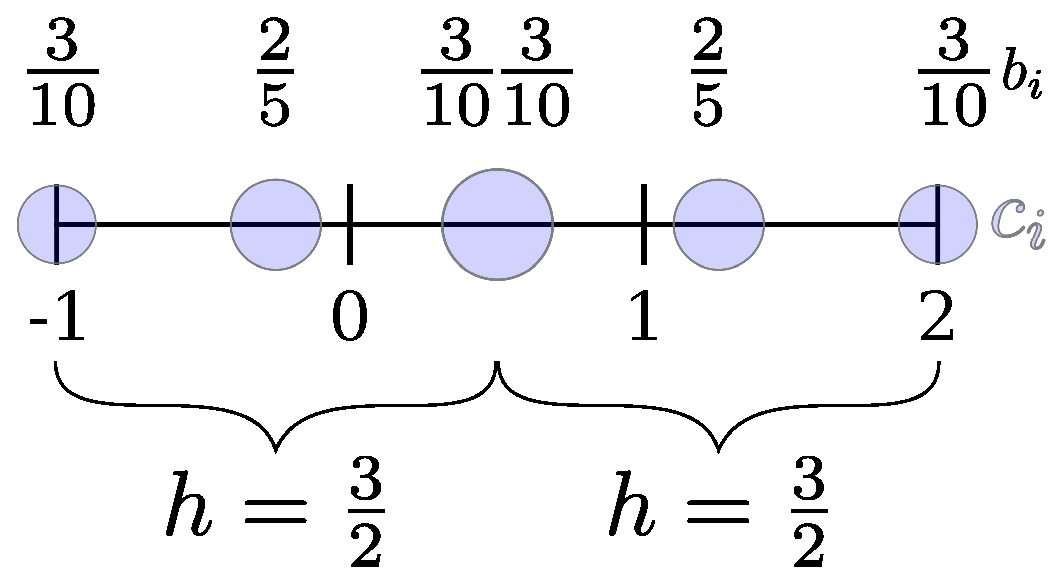
\includegraphics[scale=0.29]{T13}
       \end{figure}\\ 
       Python 3.5
       \begin{mdframed}[linewidth=0pt,backgroundcolor=gray!10]
	   \lstinputlisting[language=Python]{T13c.py}
	\end{mdframed}
\end{document}